%
\documentclass[12pt,letterpaper]{article}
\usepackage{bbm}
\usepackage{url}
\usepackage{float}
\usepackage{fancyhdr}
%\usepackage{fancybox}
%\usepackage{amstext}
\usepackage{amsmath}
%\usepackage{rotating}
\usepackage{multicol}
\usepackage{pictexwd}
\usepackage{enumitem}
%\usepackage{booktabs}
\usepackage{graphicx}
\usepackage{booktabs,multirow}
\usepackage{siunitx}
\usepackage{subfigure}
\setlength{\parindent}{0in}
\setlength{\textwidth}{7in}
\setlength{\evensidemargin}{-0.25in}
\setlength{\oddsidemargin}{-0.25in}
\setlength{\parskip}{.5\baselineskip}
\setlength{\topmargin}{-0.5in}
\setlength{\textheight}{9in}
%               Problem and Part
\newcounter{problemnumber}
\newcounter{partnumber}
\newcommand{\Problem}{\stepcounter{problemnumber}\setcounter{partnumber}{0}\item[\makebox{\hfil\textbf{\ \theproblemnumber.}\hfil}]}
\newcommand{\Part}{\stepcounter{partnumber}\item[(\alph{partnumber})]}
\newcommand{\SubPart}{\stepcounter{problemnumber}\setcounter{partnumber}{0}}

\pagestyle{empty}

\rhead{\large\textsc{Angeline Baniqued \& Michael Wee}}
\lhead{\LARGE\textbf{CS 181 Assignment 3}}
\cfoot{}
\renewcommand{\headrulewidth}{0.3pt}
\setlength{\headsep}{40pt}
\usepackage{amssymb}

\begin{document}

\thispagestyle{fancy}\small
  \section*{Problem 1}
  \begin{enumerate}
  \Problem
        \begin{enumerate}
        \Part
        \Part
        \Part
        \Part 
        \Part
        \end{enumerate}
  \section*{Problem 2}
  \Problem
        \begin{enumerate}
        \Part
                For the ML method, the predictive distribution is just $P(\boldsymbol{x}|\theta_{MLE})$ where you just compute the maximum likelihood estimate of the parameter
                 $\theta$ given the observed data by taking $argmax_{\theta} P(\mathcal{D}|\theta)$, and then plug it into the distribution function of the new datum. \medskip
                 
                For the MAP method, the predictive distribution is just $P(\boldsymbol{x}|\theta_{MAP})$ where you just compute the maximum a posteriori estimate of the parameter
                 $\theta$ given the observed data by taking $argmax_{\theta} P(\mathcal{D}|\theta)P(\theta)$ and then plug it into the distribution function of the new datum. \medskip
                \medskip
                
                For the FB method, the predictive distribution is just \medskip 
              
                $\displaystyle\int_\theta P(\boldsymbol{x}|\theta)P(\theta|\mathcal{D}) d\theta$ where you just get the posterior distribution $P(\theta|\mathcal{D})$, multiply it by the likelihood,
                
                $P(\boldsymbol{x}|\theta), $ and then integrate it over $\theta$. \medskip
                    
        \Part $MAP$ is more Bayesian because it makes use of the prior distribution on $\theta$ thereby treating $\theta$ as a random variable, 
           unlike $ML$ which assumes that $\theta$\ is fixed.  
        \Part 
        \Part Graphs of $Beta(1,1)$, $Beta(3,3)$, and $Beta(2,5)$ respectively  \medskip
        \begin{figure}[H]
                \centering
                \subfigure[Beta(1,1)]
                {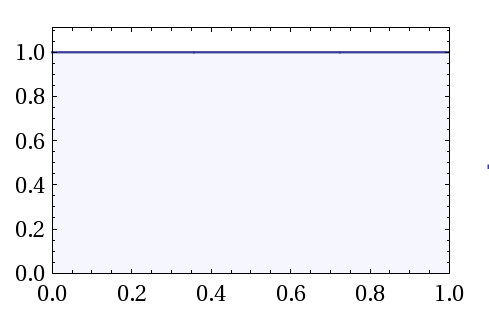
\includegraphics[width=2.3in]{2d_beta11.png}}
                \subfigure[Beta(3,3)]
                {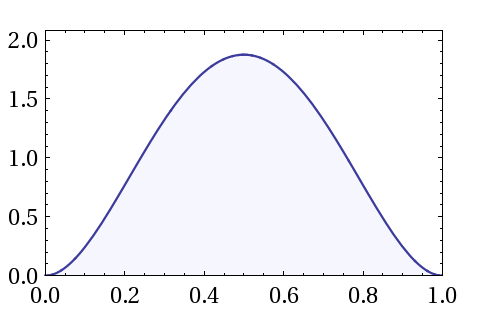
\includegraphics[width=2.3in]{2d_beta33.png}}
                \subfigure[Beta(2,5)]
                {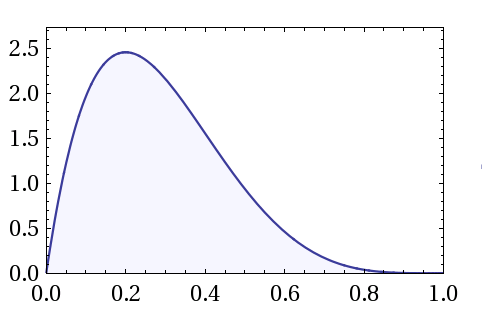
\includegraphics[width=2.3in]{2d_beta25.png}}
        \end{figure}            
        The intuition behind using a $Beta(\alpha, \beta)$ model is to denote the number of wins or losses by the soccer team. We can think of $ \alpha$ as the number of
        success and $\beta$ as the number of losses. It makes sense to use a $Beta$ distribution as a prior for the probability of a win because the expected value of a $Beta$ 
        distribution is $\alpha/(\alpha+\beta)$ which is just the ratio of past wins to the total number of games the soccer team has played in the past. \medskip

In this case, if we assume a $Beta(1,1)$ prior, that's like saying the team has won once and lost once. The same reasoning holds
         for $Beta(3,3)$ and $Beta(2,5)$. Comparing the shapes of the distributions, $Beta(1,1)$ says the probability of winning is uniformly distributed from $[0,1]$. $Beta(3,3)$ shows 
         that the probability of winning is concentrated near $0.5$. $Beta(2,5)$ shows that the probability of winning is skewed to the right because given a past record of 2-5 wins to losses, the probability of winning
        should be pretty low. 
        \Part The $Beta$ distribution is useful when used with MAP estimation for reasoning with Bernoulli (binary) R.V.s because the $Beta$ distribution is the conjugate prior 
        of a Bernoulli. \medskip
        \Part Based on $http://www.gocrimson.com/sports/fball/2011-12/schedule$, the Harvard football team won 9 times and lost once in the 2011-2012 season. Also, they won  the first 3 games of the 2012-2013 season. Given this history, $\mathcal{D} = \{1,1,1\}$.\medskip
        
                \begin{enumerate}[ref=(\roman{*})]
                 \item For the ML estimation, solve for $argmax_{\theta} P(\mathcal{D}|\theta).$   \medskip \\
        
            $P(\mathcal{D}|\theta) = \displaystyle \prod_{i=1}^{N} \theta^{\mathcal{D}_i}(1-\theta)^{1-\mathcal{D}_i}= \theta^{\sum\mathcal{D}_i}  (1-\theta)^{N-\sum\mathcal{D}_i}  $ where $N$ is the number of data in $\mathcal{D}$. \medskip
            
            $ log P(\mathcal{D}|\theta)  = \displaystyle \sum{\boldsymbol{D}_i}log(\theta) +\displaystyle (N-\boldsymbol{\sum D}_i)log(1-\theta)$\medskip
            
            $  \displaystyle\frac{\partial{log(P(\mathcal{D}|\theta))}}{\partial{\theta}} =  \displaystyle \frac{\sum{\boldsymbol{D}_i}}{\theta} -  \frac{N-\sum{\boldsymbol{D}_i}}{1- \theta} = 0$ \medskip 
            
            Solving for $\theta$, we get $\theta_{MLE} = \displaystyle \frac{\sum{\boldsymbol{D}_i}}{N} = 3/3 = 1.  $ Probability of winning the next game is 1. \medskip \\
            
        
                \item For the $MAP$  estimation, we'll use the prior $Beta(9,1)$ and we'll solve \medskip
                
                 $argmax_{\theta} P(\mathcal{D}|\theta)P(\theta).$ \medskip
                
                $P(\mathcal{D}|\theta)P(\theta)=\displaystyle\left(  \prod_{i=1}^{N} \theta^{\mathcal{D}_i}(1-\theta)^{1-\mathcal{D}_i} \right)\frac{\theta^{9-1}(1-\theta)^{1-1}}{\Gamma(9,1)}$ \\
                
               $ \propto \displaystyle\left(  \prod_{i=1}^{N} \theta^{\mathcal{D}_i}(1-\theta)^{1-\mathcal{D}_i} \right)\theta^{8} =  \theta^{\sum\mathcal{D}_i}  (1-\theta)^{N-\sum\mathcal{D}_i}\theta^{8}}  $ \medskip
 
                $\propto   \theta^{8+\sum\mathcal{D}_i}  (1-\theta)^{N-\sum\mathcal{D}_i}$  \medskip
                
                $ log(P(\mathcal{D}|\theta)P(\theta)) =  (8+\sum\mathcal{D}_i)log(\theta) + (N-\sum\mathcal{D}_i)log(1-\theta) $ \medskip
                
                $  \displaystyle\frac{\partial{log(P(\mathcal{D}|\theta)P(\theta))}}{\partial{\theta}} =  \frac{(8+\sum\mathcal{D}_i)}{\theta}-  \frac{(N-\sum\mathcal{D}_i)}{1-\theta} = 0$
                
                Solving for $\theta$, we get $\theta_{MAP} = \displaystyle \frac{8+\sum{\boldsymbol{D}_i}}{N+8} = (8+3)/(3+8) = 1   $ \medskip
                
                Probability of winning the next game is 1.\bigskip
                
                \item  For the $Fully  Bayesian$  estimation, we'll again use the prior $Beta(9,1).$ \medskip
                
                $P(x=1|\mathcal{D}) = \displaystyle \int_{0}^1P(x=1|\theta)P(\theta)d\theta$ \medskip
                   
                 $P(\mathcal{D}|\theta)P(\theta)=\displaystyle\left(  \prod_{i=1}^{N} \theta^{\mathcal{D}_i}(1-\theta)^{1-\mathcal{D}_i} \right)\frac{\theta^{9-1}(1-\theta)^{1-1}}{\Gamma(9,1)}$ \\
                
               $ \propto \displaystyle\left(  \prod_{i=1}^{N} \theta^{\mathcal{D}_i}(1-\theta)^{1-\mathcal{D}_i} \right)\theta^{8} =  \theta^{\sum\mathcal{D}_i}  (1-\theta)^{N-\sum\mathcal{D}_i}\theta^{8}}  $ \medskip
 
                $\propto   \theta^{8+\sum\mathcal{D}_i}  (1-\theta)^{N-\sum\mathcal{D}_i}      $ \\
                
                From here, we can transform this into a $Beta(9+\sum\mathcal{D}_i,N-\sum\mathcal{D}_i+1) $ by multiplying and dividing the expression by a proportionality constant so that when we do the integration, the PDF\ of that beta distribution just becomes 1. The integration basically computes $\mathbb{E}(\theta|\mathcal{D)}$ and since we know that the expected value of $Beta(\alpha,\beta) $ is $\alpha/(\alpha+\beta)$, the probability of winning the next game is just $\displaystyle \frac{(9+\sum\mathcal{D}_i)}{(N-\sum\mathcal{D}_i+1+9+\sum\mathcal{D}_i)}=\frac{9+3}{3+10}\approx 0.92.\ $ \medskip
                \medskip
                
                Probability of winning the next game is 0.92.

                \end{enumerate} \bigskip
       \end{enumerate}
  \section*{Problem 3}
  \Problem
        \begin{enumerate}
        \Part
        \Part
        \end{enumerate}
  \section*{Problem 4}
  \Problem
        \begin{enumerate}
        \Part $K$-means clustering algorithm
                \begin{enumerate}
                        \item Plot of the number of clusters $K$ vs. mean squared error \\
                                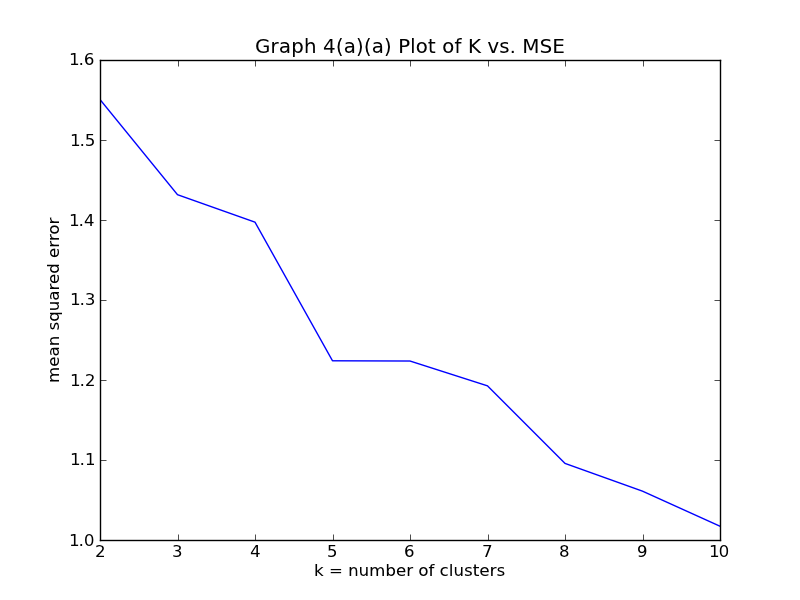
\includegraphics[width=3.5in]{4aa.png}
                        \item
                \end{enumerate}
        \Part $HAC$ clustering algorithm \medskip
        
        (a)\medskip 
                \begin{enumerate}
                        
                        \item For the minimum distance metric: \medskip \\
                        
                        \begin{tabular}{@{}l | c |  c|  c |  c} \hline \hline  \\ [-2ex]
         & $  Cluster 1  $ & $Cluster 2$ &  $Cluster3$ & $Cluster4$ \\ \hline  \noalign{\smallskip}
      Number of instances   & 1     & 1   & 25  &73  \\ \hline \hline

                        \end{tabular}
                        \begin{figure}[H]
                                \centering
                                \caption{Minimum distance metric (x-axis: age, y-axis:\ education, z-axis: income)} {
                                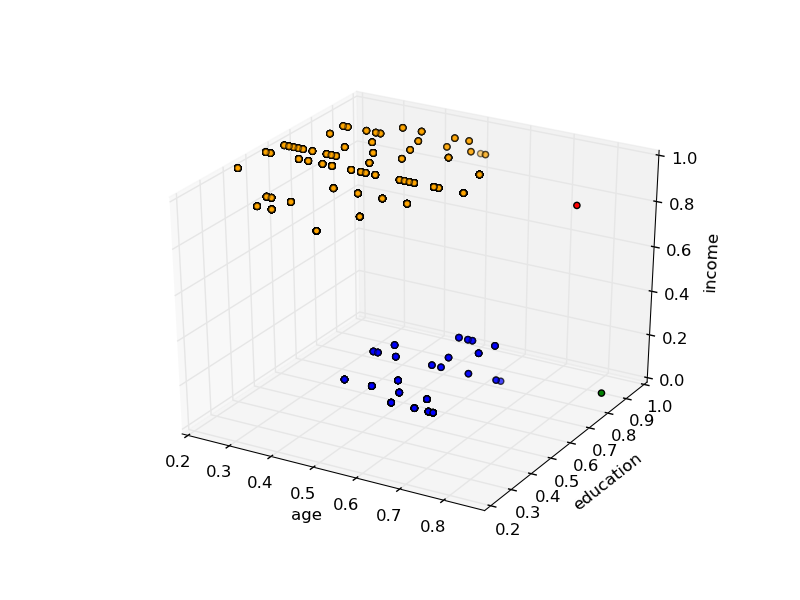
\includegraphics[width=3.5in]{4ba_min.png} }\\
                        \end{figure}
                        \item  For the maximum distance metric: \medskip
                        
                        \begin{tabular}{@{}l | c |  c|  c |  c} \hline \hline  \\ [-2ex]
         & $  Cluster 1  $ & $Cluster 2$ &  $Cluster3$ & $Cluster4$ \\ \hline  \noalign{\smallskip}
      Number of instances   & 19     & 23   & 32  &26  \\ \hline \hline

                        \end{tabular}
                        \begin{figure}[H]
                                \centering
                                \caption{Minimum distance metric (x-axis: age, y-axis:\ education, z-axis: income)} {
                                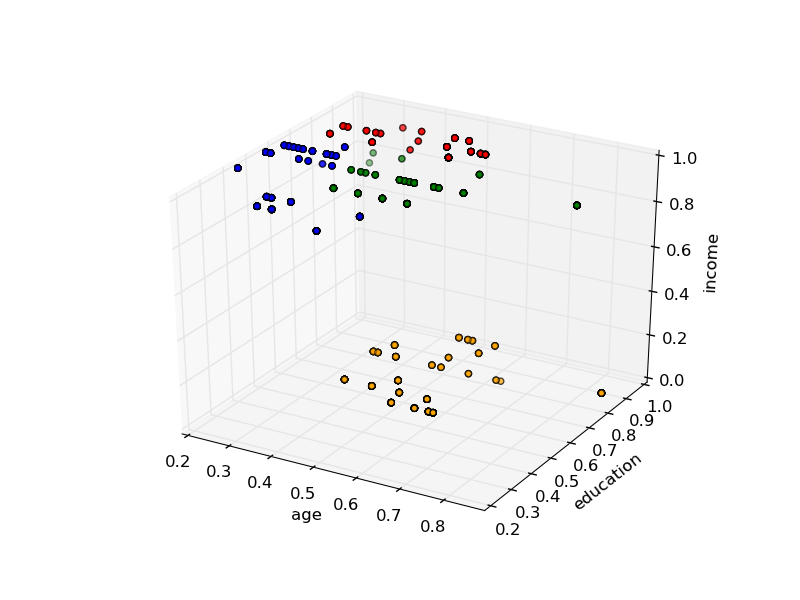
\includegraphics[width=3.5in]{4ba_max.png} }\\
                        \end{figure}
                \end{enumerate}
           (b)\medskip 
           
            \begin{enumerate}
                        
                        \item For the mean distance metric: \medskip \\
                        
                        \begin{tabular}{@{}l | c |  c|  c |  c} \hline \hline  \\ [-2ex]
         & $  Cluster 1  $ & $Cluster 2$ &  $Cluster3$ & $Cluster4$ \\ \hline  \noalign{\smallskip}
      Number of instances   & 1     & 9   & 143  &47  \\ \hline \hline

                        \end{tabular}
                        \begin{figure}[H]
                                \centering
                                \caption{Mean distance metric (x-axis: age, y-axis:\ education, z-axis: income)} {
                                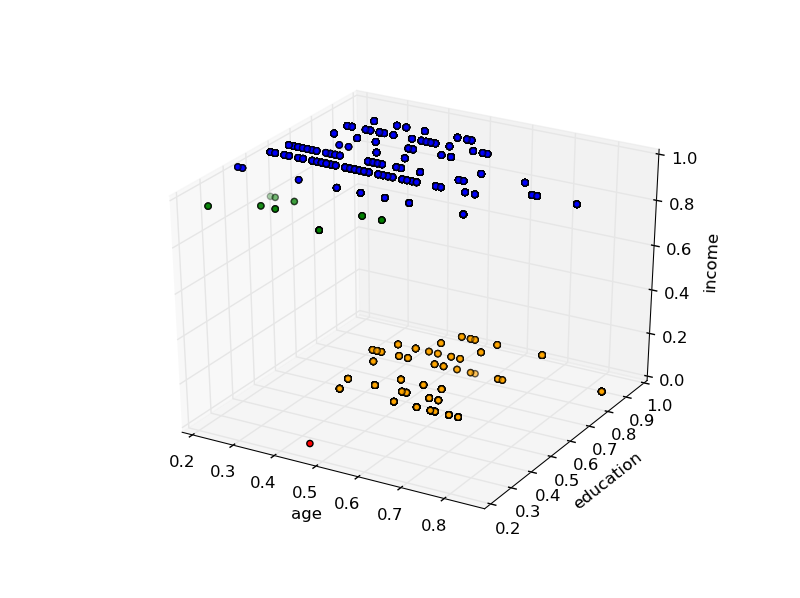
\includegraphics[width=3.5in]{4bb_mean.png} }\\
                        \end{figure}
                        \item  For the centroid distance metric: \medskip
                        
                        \begin{tabular}{@{}l | c |  c|  c |  c} \hline \hline  \\ [-2ex]
         & $  Cluster 1  $ & $Cluster 2$ &  $Cluster3$ & $Cluster4$ \\ \hline  \noalign{\smallskip}
      Number of instances   & 1     & 5   & 147  &47  \\ \hline \hline

                        \end{tabular}
                        \begin{figure}[H]
                                \centering
                                \caption{Centroid distance metric (x-axis: age, y-axis:\ education, z-axis: income)} {
                                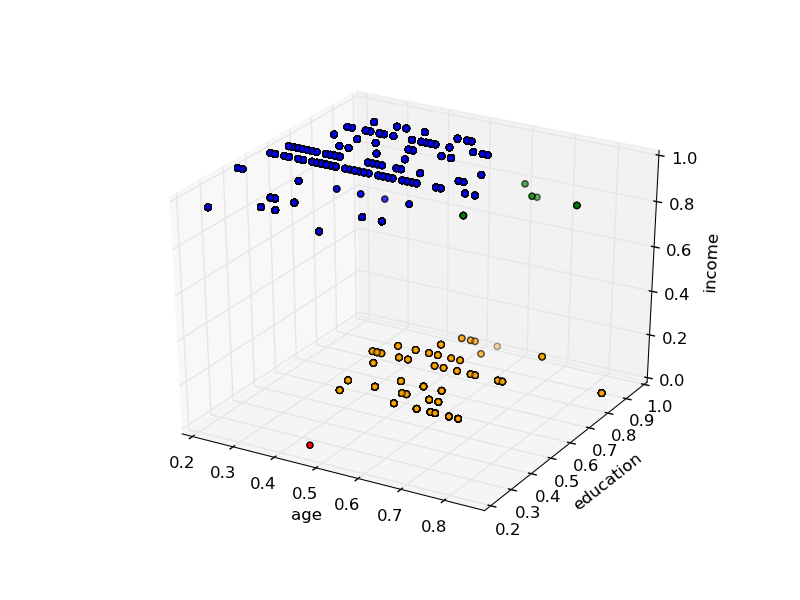
\includegraphics[width=3.5in]{4bb_cent.png} }\\
                        \end{figure}
                \end{enumerate}
        \Part
        \end{enumerate}
  \end{enumerate}
\end{document}
